\documentclass[11pt,a4paper]{article}
\usepackage[margin=2.2cm]{geometry}
\usepackage{amsmath,amssymb,amsthm,bm,graphicx,booktabs,array,enumitem,xcolor,hyperref,float,tikz}
\usetikzlibrary{positioning,arrows.meta,calc}
\hypersetup{colorlinks,linkcolor=blue!60!black,urlcolor=blue!60!black,citecolor=blue!60!black}
\newtheorem{definition}{Definition}\newtheorem{lemma}{Lemma}\newtheorem{proposition}{Proposition}\newtheorem{remark}{Remark}\newtheorem{fact}{Fact}
\setlength{\parskip}{4pt}
\newcommand{\R}{\mathbb R}
\title{\vspace{-1.2cm}The MLP of $t$ and the Fourier MLP\\[2pt]\large shapes, parameter counts, and why the input representation matters}
\author{Note for the paper meeting, 6 November 2026 (Joy)}
\date{}
\begin{document}
\maketitle
\vspace{-0.9cm}
\noindent\textit{Scope.} Answers to Nadia's three questions (runs, $h$, the Fourier MLP and the shapes of $w$ and $W$), written so that every count is derived and every claim about behaviour is either a stated theorem from the literature, a computation on our own fit records, or labelled as a derivation. Sections 1--3 are the direct answers; Sections 4--7 are the background she may ask about. Every number is taken from \texttt{approx\_study/fits} or recomputed from the same code; three figures (\ref{fig:units}, \ref{fig:snaps}, \ref{fig:curves}) come from a re-run of seed 0 that reproduces the stored values to all printed digits.

\section{Runs and $h$ (questions 1 and 2)}
\textbf{Runs.} Each neural model is fitted three times, seeds $\{0,1,2\}$, on identical data; reported values are means over the three, and the Excel file also gives the sample standard deviation $s=\sqrt{\tfrac1{2}\sum_{i=1}^{3}(x_i-\bar x)^2}$. A seed changes only the random initial state (initial weights; for the Fourier MLP also the drawn frequencies). For KAN~[1,1] the three seeds agree to $10^{-8}$ (Section~6 explains why); for the MLPs $s$ is of order $10^{-3}$--$10^{-2}$.

\textbf{$h$.} $h$ is the hidden width of KAN~[1,$h$,1] and is set per budget, $h=1,1,2,5,10$ for $N^*=15,30,60,120,240$. The count is $N=24h$ (Lemma~\ref{lem:kan}), so $h=1$ already gives $N=24>30$; budgets 15 and 30 therefore share one fit, 60 uses $h=2$ ($N=48$, the alternative $h=3$ giving 72), and 120, 240 are exact.

\section{The MLP of $t$: definition, shapes, count (question 3, part 1)}
\begin{definition}[two-hidden-layer MLP]
Fix $w\in\mathbb N$ and an input dimension $d$. Let $\bm W_1\in\R^{w\times d}$, $\bm b_1\in\R^{w}$, $\bm W_2\in\R^{w\times w}$, $\bm b_2\in\R^{w}$, $\bm W_3\in\R^{1\times w}$, $b_3\in\R$, and let $\tanh$ act entrywise. The network is the map $f:\R^d\to\R$,
\begin{equation}
f(\bm x)=\bm W_3\tanh\!\bigl(\bm W_2\tanh(\bm W_1\bm x+\bm b_1)+\bm b_2\bigr)+b_3 .
\label{eq:mlp}
\end{equation}
The \emph{MLP of $t$} is the case $d=1$, $\bm x=t\in[0,1]$.
\end{definition}
With $d=1$ the matrix $\bm W_1$ has $w$ rows and one column: it \emph{is} a column vector $\bm w_1=(w_{1},\dots,w_{w})^{\!\top}$, and $\bm W_1 t=t\,\bm w_1$ is the vector $(w_1 t,\dots,w_w t)^{\!\top}$. So ``a matrix multiplied by $t$'' is a vector scaled by a number; the $i$-th hidden neuron computes $\tanh(w_i t+b_i)$, an S-curve in $t$ with its own slope and centre. Figure~\ref{fig:arch} shows the data flow with every shape.

\begin{figure}[H]\centering
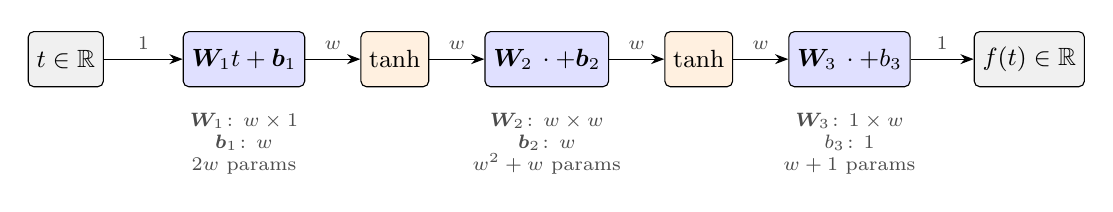
\begin{tikzpicture}[x=1cm,y=1cm,>=Stealth,font=\small,
 box/.style={draw,rounded corners=2pt,minimum height=7mm,inner sep=3pt,fill=#1!12},
 lab/.style={font=\scriptsize,text=black!70}]
\node[box=gray] (in) {$t\in\R$};
\node[box=blue,right=1.0 of in] (l1) {$\bm W_1 t+\bm b_1$};
\node[box=orange,right=0.7 of l1] (a1) {$\tanh$};
\node[box=blue,right=0.7 of a1] (l2) {$\bm W_2\,\cdot+\bm b_2$};
\node[box=orange,right=0.7 of l2] (a2) {$\tanh$};
\node[box=blue,right=0.7 of a2] (l3) {$\bm W_3\,\cdot+b_3$};
\node[box=gray,right=0.8 of l3] (out) {$f(t)\in\R$};
\draw[->] (in)--(l1) node[midway,above,lab]{$1$};
\draw[->] (l1)--(a1) node[midway,above,lab]{$w$};
\draw[->] (a1)--(l2) node[midway,above,lab]{$w$};
\draw[->] (l2)--(a2) node[midway,above,lab]{$w$};
\draw[->] (a2)--(l3) node[midway,above,lab]{$w$};
\draw[->] (l3)--(out) node[midway,above,lab]{$1$};
\node[below=2mm of l1,lab,align=center]{$\bm W_1\!:\,w\times1$\\$\bm b_1\!:\,w$\\ $2w$ params};
\node[below=2mm of l2,lab,align=center]{$\bm W_2\!:\,w\times w$\\$\bm b_2\!:\,w$\\ $w^2+w$ params};
\node[below=2mm of l3,lab,align=center]{$\bm W_3\!:\,1\times w$\\$b_3\!:\,1$\\ $w+1$ params};
\end{tikzpicture}
\caption{The MLP of $t$. Numbers on arrows are the dimensions of the vectors passed along; the parameters of each affine layer are listed beneath it. Total $N=w^2+4w+1$.}
\label{fig:arch}
\end{figure}

\begin{lemma}[parameter count of an affine layer]\label{lem:affine}
An affine map $\R^a\to\R^b$, $\bm x\mapsto \bm W\bm x+\bm b$, has exactly $ab+b=(a+1)b$ free real parameters.
\end{lemma}
\begin{proof}
$\bm W$ has $a$ columns and $b$ rows, hence $ab$ entries, and $\bm b$ has $b$ entries; the entries are independent coordinates of $\R^{ab+b}$. The activations $\tanh$ have no parameters.
\end{proof}

\begin{proposition}[count for the MLP of $t$]\label{prop:mlp}
With $d=1$ and both hidden layers of width $w$, $N_{\mathrm{MLP}}(w)=w^2+4w+1$.
\end{proposition}
\begin{proof}
Apply Lemma~\ref{lem:affine} to the three layers, $(a,b)=(1,w),(w,w),(w,1)$: $(1+1)w+(w+1)w+(w+1)\cdot1=2w+w^2+w+w+1=w^2+4w+1$.
\end{proof}
Hence $w=2,4,6,9,14$ give $N=13,33,61,118,253$. The map $w\mapsto N$ is strictly increasing and quadratic, so between consecutive admissible values there are gaps of $2w+5$; a budget can be met exactly only if $N^*-1$ happens to be of the form $w^2+4w$, which none of $15,30,60,120,240$ is. Figure~\ref{fig:counts} shows the admissible counts against the budgets.

\section{The Fourier MLP (question 3, part 2)}
\begin{definition}[random Fourier features]\label{def:rff}
Fix $m\in\mathbb N$ and $\sigma>0$. Draw $b_1,\dots,b_m\overset{\text{iid}}\sim\mathcal N(0,\sigma^2)$ once and keep them fixed. The feature map is
\begin{equation}
\bm\gamma:[0,1]\to\R^{2m},\qquad
\bm\gamma(t)=\bigl(\sin 2\pi b_1t,\dots,\sin 2\pi b_mt,\ \cos 2\pi b_1t,\dots,\cos 2\pi b_mt\bigr)^{\!\top}.
\label{eq:gamma}
\end{equation}
The \emph{Fourier MLP} is the network of Definition~1 with $d=2m$ applied to $\bm x=\bm\gamma(t)$, i.e.\ $f_{\mathrm F}(t)=f(\bm\gamma(t))$. In the study $\sigma=6$ and the $b_j$ are drawn once per seed.
\end{definition}
The $b_j$ are \emph{not} parameters of the model in the optimisation sense (they are never updated) and are not counted; one may regard them as part of the architecture, like the choice of $\tanh$.

\begin{proposition}[count for the Fourier MLP]\label{prop:fmlp}
$N_{\mathrm{FMLP}}(m,w)=w^2+(2m+3)w+1$.
\end{proposition}
\begin{proof}
Only the first layer changes: $(a,b)=(2m,w)$ contributes $(2m+1)w$ by Lemma~\ref{lem:affine}; the other two layers contribute $w^2+w$ and $w+1$ as before. Sum: $2mw+w+w^2+w+w+1$.
\end{proof}
Thus $(m,w)=(2,2),(2,3),(4,4),(6,6),(8,9)$ give $N=19,31,61,127,253$ (e.g.\ $(4,4)$: $16+11\cdot4+1=61$). Two integers are free, so the admissible set is denser than for the plain MLP (Figure~\ref{fig:counts}), which is why this model lands closer to the budgets.

\begin{figure}[H]\centering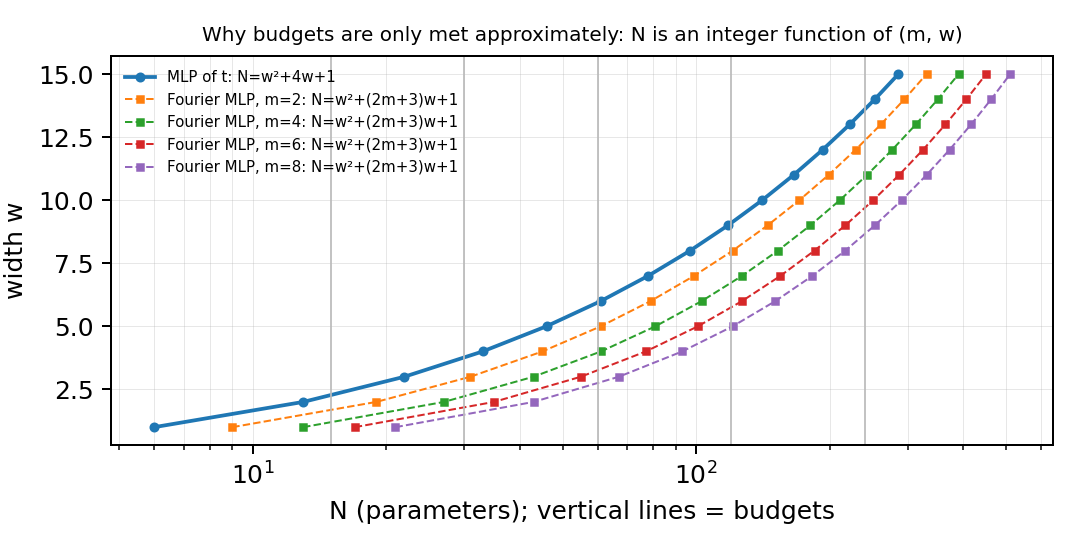
\includegraphics[width=.78\textwidth]{fig_counts.png}
\caption{Admissible parameter counts. Each curve is $w\mapsto N$ for one architecture; the vertical lines are the budgets. The plain MLP has one curve and must take the nearest point on it; the Fourier MLP has one curve per $m$ and can pick the closest point across them.}
\label{fig:counts}
\end{figure}

\begin{figure}[H]\centering
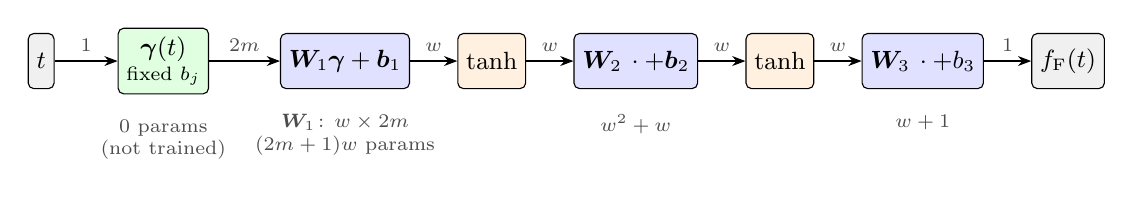
\begin{tikzpicture}[x=1cm,y=1cm,>=Stealth,font=\small,
 box/.style={draw,rounded corners=2pt,minimum height=7mm,inner sep=3pt,fill=#1!12},
 lab/.style={font=\scriptsize,text=black!70}]
\node[box=gray] (in) {$t$};
\node[box=green,right=0.8 of in,align=center] (g) {$\bm\gamma(t)$\\[-2pt]{\scriptsize fixed $b_j$}};
\node[box=blue,right=0.9 of g] (l1) {$\bm W_1\bm\gamma+\bm b_1$};
\node[box=orange,right=0.6 of l1] (a1) {$\tanh$};
\node[box=blue,right=0.6 of a1] (l2) {$\bm W_2\,\cdot+\bm b_2$};
\node[box=orange,right=0.6 of l2] (a2) {$\tanh$};
\node[box=blue,right=0.6 of a2] (l3) {$\bm W_3\,\cdot+b_3$};
\node[box=gray,right=0.6 of l3] (out) {$f_{\mathrm F}(t)$};
\draw[->] (in)--(g) node[midway,above,lab]{$1$};
\draw[->] (g)--(l1) node[midway,above,lab]{$2m$};
\draw[->] (l1)--(a1) node[midway,above,lab]{$w$};
\draw[->] (a1)--(l2) node[midway,above,lab]{$w$};
\draw[->] (l2)--(a2) node[midway,above,lab]{$w$};
\draw[->] (a2)--(l3) node[midway,above,lab]{$w$};
\draw[->] (l3)--(out) node[midway,above,lab]{$1$};
\node[below=2mm of g,lab,align=center]{$0$ params\\(not trained)};
\node[below=2mm of l1,lab,align=center]{$\bm W_1\!:\,w\times2m$\\$(2m+1)w$ params};
\node[below=2mm of l2,lab,align=center]{$w^2+w$};
\node[below=2mm of l3,lab,align=center]{$w+1$};
\end{tikzpicture}
\caption{The Fourier MLP: identical to Figure~\ref{fig:arch} except for the fixed feature map in front, which widens the first layer from $1$ to $2m$ inputs.}
\end{figure}

\begin{figure}[H]\centering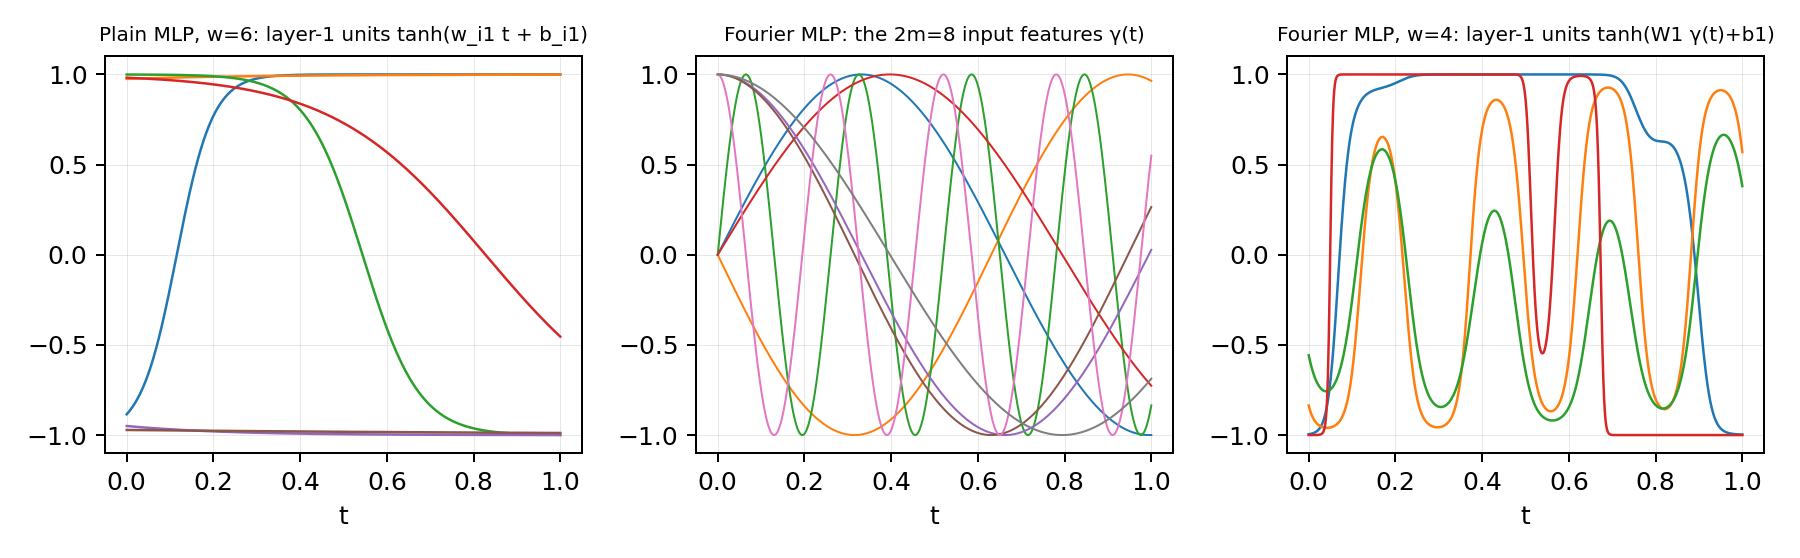
\includegraphics[width=\textwidth]{fig_units.png}
\caption{What each network has to work with (CBA, seed 0, budget 60, after training). Left: the six layer-1 units of the plain MLP are monotone S-curves of $t$; everything the network outputs is a smooth recombination of these. Middle: the eight fixed inputs of the Fourier MLP already oscillate. Right: the four layer-1 units of the Fourier MLP are mixtures of those oscillations.}
\label{fig:units}
\end{figure}

\section{Why the input representation matters: two theorems and one identity}
Both networks can, in principle, represent any continuous target:
\begin{fact}[universal approximation; Cybenko 1989, Hornik 1991]
For any continuous $g:[0,1]\to\R$ and $\varepsilon>0$ there is a one-hidden-layer network with sigmoidal (e.g.\ $\tanh$) units and some finite width such that $\sup_{t}|g(t)-f(t)|<\varepsilon$.
\end{fact}
The theorem is silent about two things that decide our experiment: how large $w$ must be for a given $\varepsilon$, and whether gradient descent finds those weights. The second is where the plain MLP loses.

\begin{fact}[spectral bias; Rahaman et al.\ 2019]\label{fact:sb}
For networks trained by gradient descent, the Fourier components of the fitted function are learned at rates that decrease with frequency: low-frequency content of the target is fitted first and high-frequency content only after much longer training. Rahaman et al.\ prove, for ReLU networks, that the Fourier transform of the network output decays at least as fast as $O(k^{-\Delta-1})$ in the frequency $k$ for some $\Delta\ge1$ determined by the depth, and that the gradient-flow dynamics inherit this ordering; they confirm the same qualitative behaviour empirically for other activations, including $\tanh$.
\end{fact}
The cleanest modern statement uses the neural tangent kernel (Jacot et al.\ 2018): in the wide-network limit, gradient flow on the squared loss makes the residual $r(\tau)=f_\tau-g$ (as a vector over the training points) evolve as $r(\tau)=e^{-\tau K}r(0)$, where $K$ is the tangent kernel matrix. Writing $r(0)=\sum_i c_i\bm v_i$ in the eigenbasis of $K$, each component decays as $e^{-\tau\lambda_i}$. For an input that is a scalar $t$ fed through smooth activations, $K$ is dominated by slowly varying eigenvectors with large $\lambda_i$, while oscillatory eigenvectors have tiny $\lambda_i$ and their residual components barely move in $20{,}000$ steps. Figure~\ref{fig:snaps} (left) is exactly this picture: the trend is in place after 200 steps, the detail is still missing after $20{,}000$.

\begin{figure}[H]\centering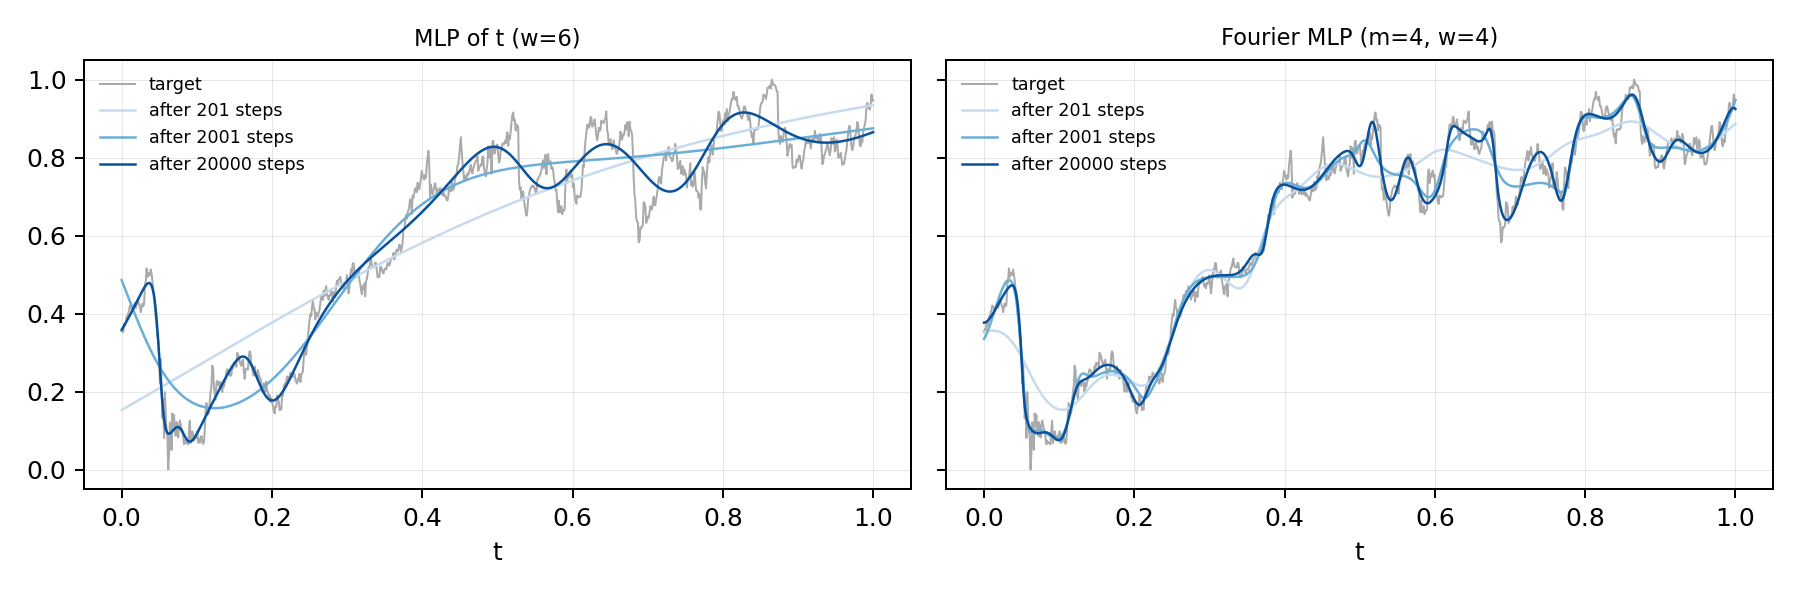
\includegraphics[width=\textwidth]{fig_snaps.png}
\caption{Fitted function after 201, 2001 and 20{,}000 Adam steps (CBA, seed 0, $N=61$ for both). Left, MLP of $t$: low frequencies first, high frequencies never. Right, Fourier MLP: the oscillatory structure is present early and is refined.}
\label{fig:snaps}
\end{figure}

What the Fourier features change is the kernel, and the mechanism is an elementary identity.
\begin{proposition}[the feature map is stationary]\label{prop:stat}
For $\bm\gamma$ as in \eqref{eq:gamma}, $\ \bm\gamma(t)^{\!\top}\bm\gamma(t')=\sum_{j=1}^{m}\cos\bigl(2\pi b_j(t-t')\bigr)$, a function of $t-t'$ only.
\end{proposition}
\begin{proof}
For each $j$, $\sin a\sin a'+\cos a\cos a'=\cos(a-a')$ with $a=2\pi b_jt$, $a'=2\pi b_jt'$; sum over $j$.
\end{proof}
\begin{proposition}[expected kernel is Gaussian; Rahimi \& Recht 2007]\label{prop:rr}
If $b\sim\mathcal N(0,\sigma^2)$ then\[\mathbb E\bigl[\cos 2\pi b\Delta\bigr]=\exp(-2\pi^2\sigma^2\Delta^2).\] Hence $\tfrac1m\bm\gamma(t)^{\!\top}\bm\gamma(t')$ is an unbiased Monte-Carlo estimate, with $m$ samples, of the Gaussian kernel $k(t,t')=\exp\!\bigl(-\tfrac{(t-t')^2}{2\ell^2}\bigr)$ with length-scale $\ell=\dfrac{1}{2\pi\sigma}$.
\end{proposition}
\begin{proof}
$\mathbb E[\cos 2\pi b\Delta]=\operatorname{Re}\,\mathbb E[e^{i2\pi\Delta b}]$, the real part of the characteristic function of $\mathcal N(0,\sigma^2)$ at $2\pi\Delta$, which is $e^{-\frac12\sigma^2(2\pi\Delta)^2}=e^{-2\pi^2\sigma^2\Delta^2}$. Matching $e^{-\Delta^2/(2\ell^2)}$ gives $\ell^{-2}=4\pi^2\sigma^2$.
\end{proof}
Tancik et al.\ (2020) combine these two facts with the NTK: composing the network with $\bm\gamma$ turns its tangent kernel into a \emph{stationary} kernel whose spectrum is controlled by $\sigma$, so that frequencies up to roughly $\sigma$ (in cycles over $[0,1]$) acquire eigenvalues large enough to be learned quickly. With $\sigma=6$, $\ell=1/(2\pi\cdot6)\approx0.0265$ of the series, i.e.\ about $24$ trading days of the 901: the network is being told that prices a month apart are related and prices a year apart need not be. Figure~\ref{fig:kernel} shows the Monte-Carlo kernel for $m=2,8,200$ against the Gaussian limit; at $m=2$ (budgets 15 and 30) the estimate is very rough, which is the rigorous reason the Fourier MLP is unreliable at the two smallest budgets and has the largest seed-to-seed spread there ($s=0.037$ at CBA, 15).

\begin{figure}[H]\centering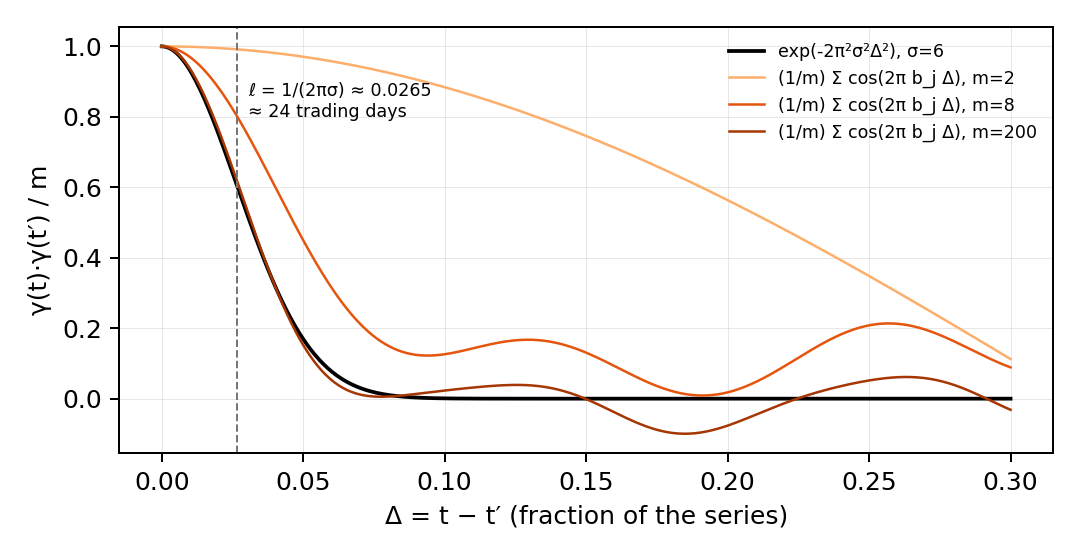
\includegraphics[width=.72\textwidth]{fig_kernel.png}
\caption{Proposition~\ref{prop:rr} in a picture: the inner product of the feature vectors at two times, averaged over the $m$ frequencies, against the time difference $\Delta$. With many frequencies it is the Gaussian bump of width $\ell$; with $m=2$ it is a poor estimate.}
\label{fig:kernel}
\end{figure}

\begin{figure}[H]\centering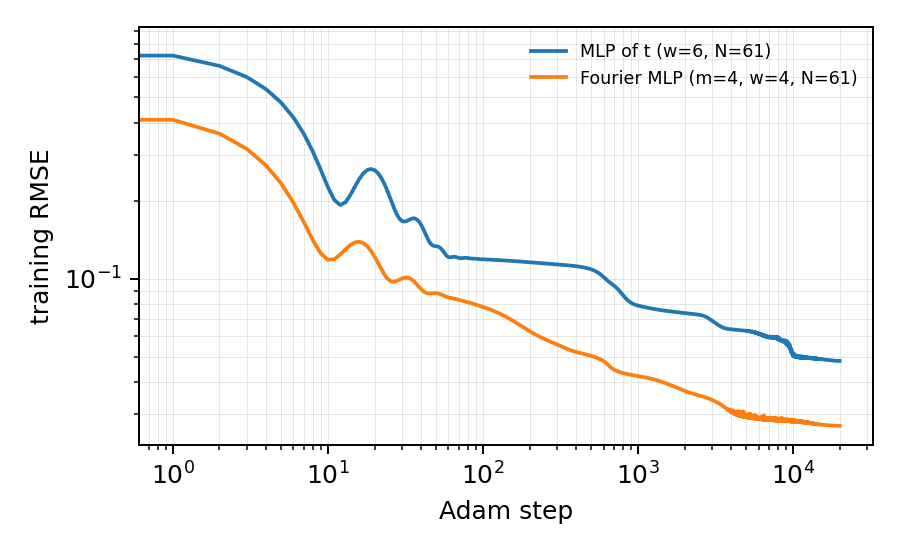
\includegraphics[width=.6\textwidth]{fig_curves.png}
\caption{Training RMSE against step for the two $61$-parameter networks (CBA, seed 0). Final values $0.0482$ and $0.0271$, identical to the stored fits. The Fourier MLP is below the plain MLP from the first hundred steps on.}
\label{fig:curves}
\end{figure}

\section{Reading the result in the frequency domain}
If Fact~\ref{fact:sb} is the explanation, the unfitted part of the series should be its high-frequency part for the plain MLP and much less so for the others. Figure~\ref{fig:spectrum} takes the residual $y-\hat f$ of the best seed at budget 60 and plots its discrete Fourier amplitude. The plain MLP's residual coincides with the target's own spectrum above about 10 cycles: it has not fitted anything there. The Fourier MLP and the KAN~[1,1] remove roughly an order of magnitude more amplitude between 5 and 40 cycles and leave only the day-to-day noise, which no $60$-parameter model should fit.

\begin{figure}[H]\centering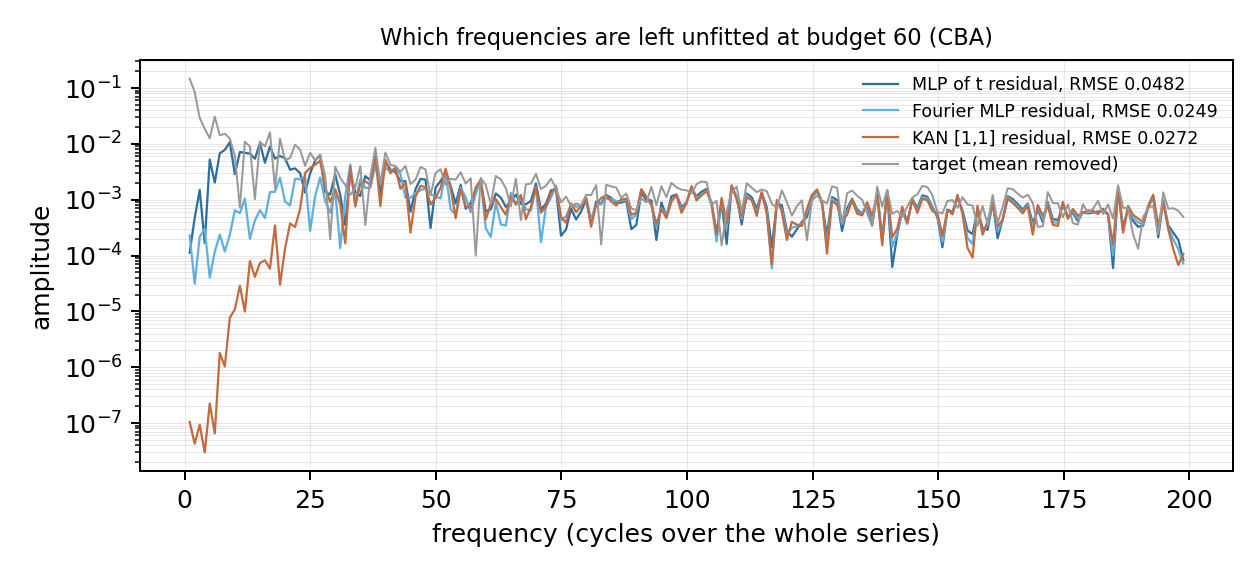
\includegraphics[width=.82\textwidth]{fig_spectrum.png}
\caption{Amplitude spectrum of the fitting residual at budget 60 (CBA, best seed), with the target's spectrum in grey. Frequency is in cycles over the whole 3.5-year series.}
\label{fig:spectrum}
\end{figure}

\section{The KAN~[1,1] as the yardstick}
\begin{lemma}[KAN parameter counts]\label{lem:kan}
In PyKAN with spline degree $k$ and grid size $G$, every edge carries $G+k$ spline coefficients, two scale weights ($w_b$ for the base function, $w_s$ for the spline) and four affine parameters of a symbolic branch that is inactive but trainable. Hence a [1,1] network has $N=G+k+6=G+9$ parameters for $k=3$, and a [1,$h$,1] network with $G=3$ has $2h$ edges and $N=2h\cdot12=24h$.
\end{lemma}
\begin{proof}
A cubic B-spline space on $G$ equal subintervals of an interval with the standard clamped knot vector has dimension $G+k$ (de Boor 2001, Ch.~IX). The remaining counts are read off the library's parameter list; the totals were verified against \texttt{sum(p.numel() for p in net.parameters() if p.requires\_grad)} for every fit: $15,30,60,120,240$ and $24,24,48,120,240$.
\end{proof}

\begin{proposition}[a [1,1] KAN is a least-squares spline]\label{prop:ls}
A [1,1] KAN computes $f(t)=w_b\,\mathrm{silu}(t)+w_s\sum_{i=1}^{G+3}c_iB_i(t)$ with $B_i$ the cubic B-splines on the fixed grid. The set of functions it can represent is the linear space $V=\operatorname{span}\{\mathrm{silu},B_1,\dots,B_{G+3}\}$, and the minimum of $\sum_n(f(t_n)-y_n)^2$ over $V$ is attained at a unique $f^\star\in V$ whenever the design matrix $[\mathrm{silu}(t_n)\ B_i(t_n)]$ has full column rank, which holds here (901 equispaced points, at most 231 intervals, so every B-spline support contains data; Schoenberg--Whitney).
\end{proposition}
\begin{proof}
Representability: the parametrisation $(w_s,c_i)\mapsto w_sc_i$ is onto $\R^{G+3}$, so the image is all of $V$. Uniqueness: the squared loss is a strictly convex quadratic in the coefficients of $V$ when the design matrix has full column rank, hence has one minimiser; different $(w_s,c)$ giving the same $w_sc$ are the same function.
\end{proof}
This is why KAN~[1,1] has zero seed-to-seed spread and why it matches a textbook least-squares spline: refitting an \texttt{LSQUnivariateSpline} on the same $G$ for each budget gives the same RMSE to five decimals and a maximum pointwise difference of $1.4\times10^{-4}$ (Figure~\ref{fig:spline}). It is a classical object in KAN clothing, and that is what makes it the right yardstick for the MLPs.

\begin{figure}[H]\centering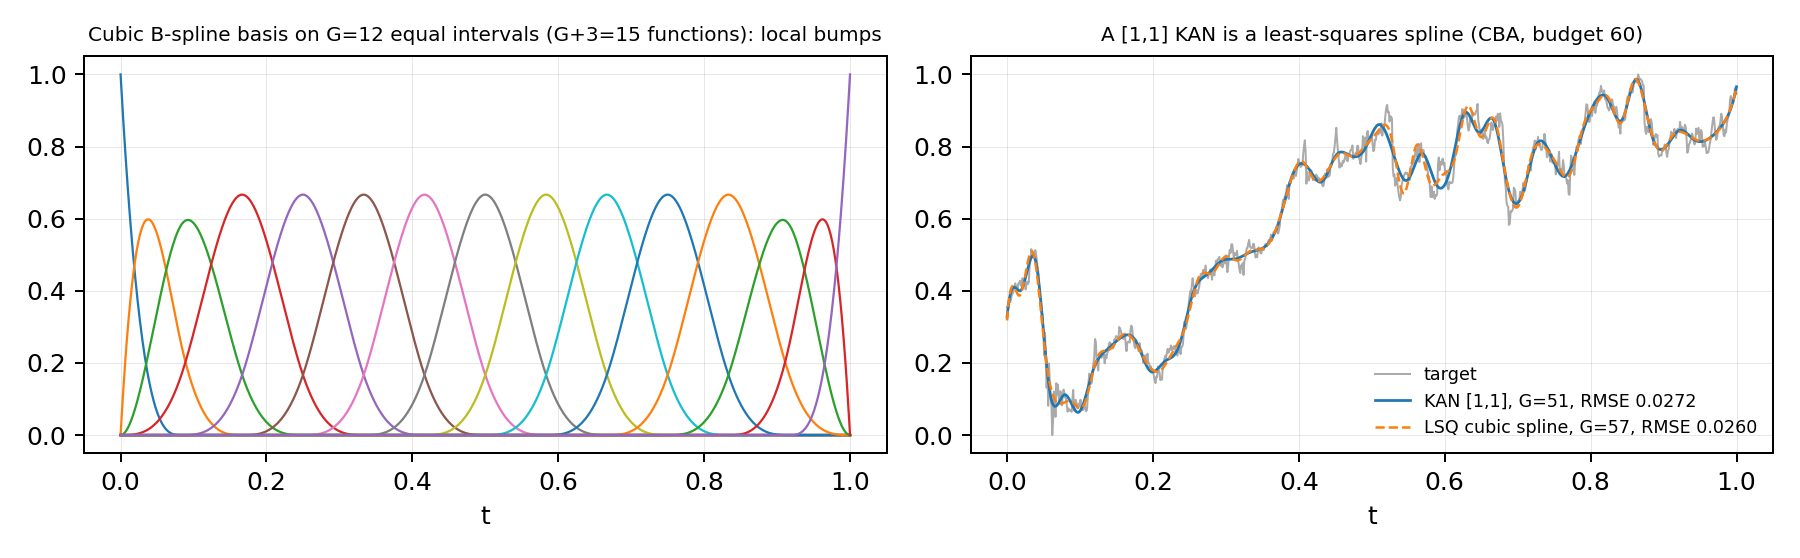
\includegraphics[width=\textwidth]{fig_spline.png}
\caption{Left: the cubic B-spline basis for $G=12$: local bumps, each non-zero on four subintervals. Right: KAN~[1,1] and a least-squares cubic spline at budget 60 on CBA (different $G$ here, 51 vs 57; at equal $G$ they coincide to $10^{-4}$).}
\label{fig:spline}
\end{figure}

\section{Error against size: the rates}
\textbf{What theory predicts (derivation, not a theorem about our data).} A Brownian path is Hölder continuous of every order $\alpha<\tfrac12$ and of no order $\alpha>\tfrac12$ (Lévy's modulus of continuity). Jackson-type theorems for splines (de Boor 2001; DeVore \& Lorentz 1993, Ch.~7 and~12) give, for an $\alpha$-Hölder target and $n$ free coefficients, best-approximation error $O(n^{-\alpha})$ in $L_2$ as well as in $L_\infty$, and this rate is sharp for the class. If daily closes behave like a rough path of this kind, a well-fitted spline, and anything equivalent to one, should show RMSE $\propto N^{-1/2}$ on a log-log plot, i.e.\ a slope near $-0.5$.

\textbf{What we measure.} Fitting $\log\mathrm{RMSE}$ against $\log N$ over the five budgets, separately for each asset and then averaging the three slopes: KAN~[1,1] $-0.65$, Fourier MLP $-0.76$, KAN~[1,$h$,1] $-0.32$, MLP of $t$ $-0.20$ (Figure~\ref{fig:slopes}). The two fixed-basis models sit at or slightly beyond the predicted rate (the series is smoother than a pure Brownian path at the scales we resolve); the two models that must build their basis by non-convex optimisation fall well short. For the plain MLP this is not an approximation-theoretic limit: Yarotsky (2017) shows deep networks can achieve the optimal rates for Hölder classes. It is an optimisation effect, Fact~\ref{fact:sb}, and Figure~\ref{fig:spectrum} shows where the missing accuracy is.

\begin{figure}[H]\centering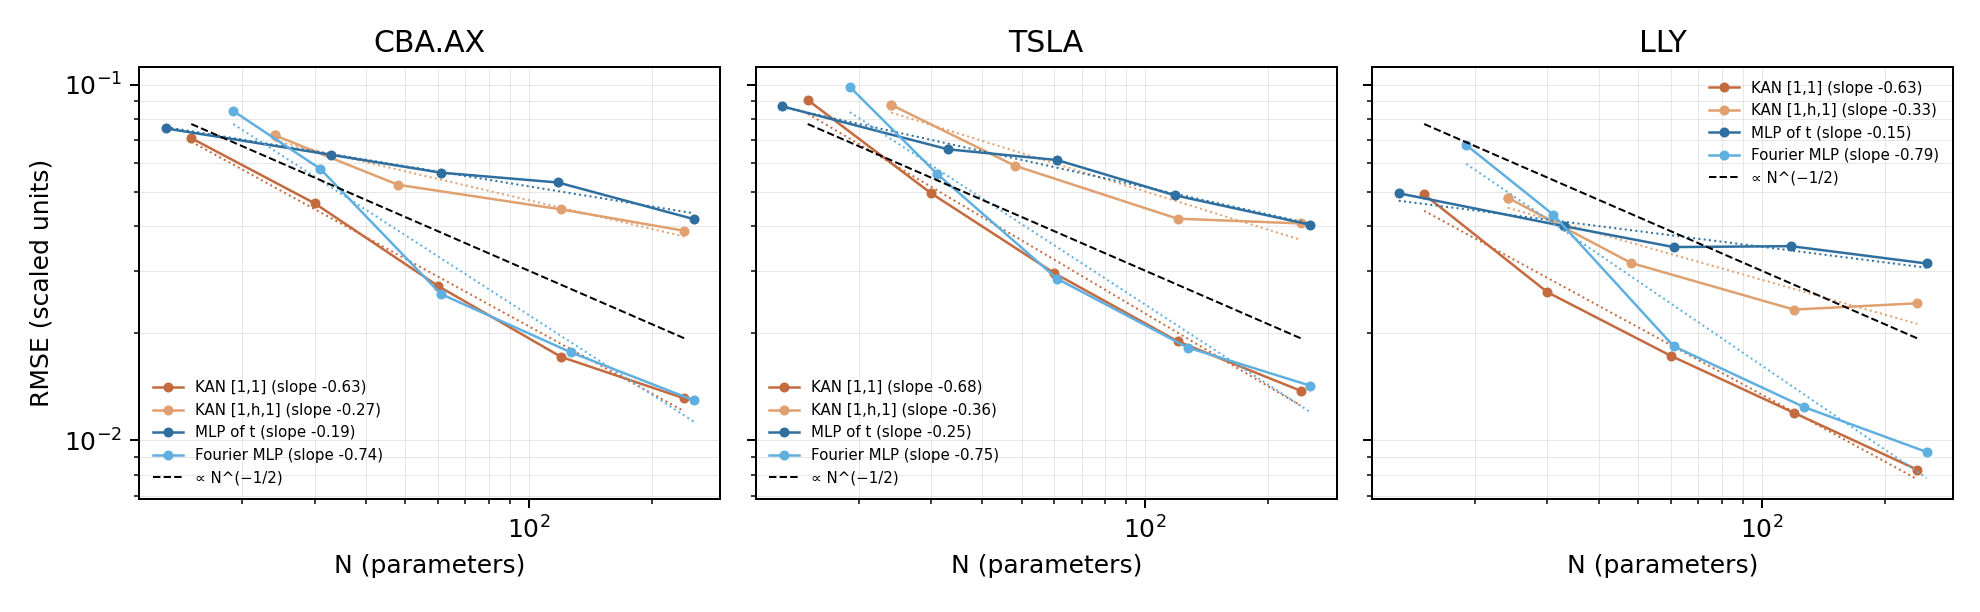
\includegraphics[width=\textwidth]{fig_slopes.png}
\caption{RMSE against actual parameter count, log-log, with the least-squares slope of each model per asset (dotted) and the $N^{-1/2}$ reference (dashed).}
\label{fig:slopes}
\end{figure}

\section{Numbers to have at hand}
\begin{table}[H]\centering\small
\caption{CBA, RMSE in scaled $[0,1]$ units, mean over 3 seeds (actual $N$ in brackets). Seed sd for KAN~[1,1] is $<10^{-7}$ at every budget.}
\begin{tabular}{lcccc}
\toprule
$N^*$ & MLP of $t$ & Fourier MLP & KAN [1,1] & KAN [1,$h$,1]\\
\midrule
15  & 0.0753 (13) & 0.0842 (19) & 0.0707 (15) & 0.0720 (24)\\
30  & 0.0634 (33) & 0.0579 (31) & 0.0464 (30) & 0.0720 (24)\\
60  & 0.0566 (61) & 0.0258 (61) & 0.0272 (60) & 0.0523 (48)\\
120 & 0.0531 (118) & 0.0177 (127) & 0.0172 (120) & 0.0446 (120)\\
240 & 0.0419 (253) & 0.0130 (253) & 0.0131 (240) & 0.0388 (240)\\
\bottomrule
\end{tabular}
\end{table}
\begin{description}[leftmargin=0pt,itemsep=2pt]
\item[Dollar scale.] Errors are per-asset Min--Max scaled; $1.0$ = the asset's full close range. TSLA (24.08--409.97): RMSE $0.03\approx\$11.6$; LLY (119.05--468.98): $\approx\$10.5$. CBA's raw series is not in the current data set.
\item[$\sigma$.] Fixed at 6 before the runs, not tuned. One later spot check (CBA, 240): $0.0271$ at $\sigma=6$, $0.0257$ at $\sigma=20$. Larger $\sigma$ = shorter $\ell$ = finer detail reachable; a tuned Fourier MLP would be slightly better still.
\item[Steps.] 80 L-BFGS (KAN) vs 20{,}000 Adam (MLP); not comparable units, stated in the paper. KAN~[1,1] converges by 20 steps; KAN~[1,$h$,1] is under-trained at 80 (CBA, 120: $0.0447\to\approx0.037$ at 320--640); MLPs slightly under-trained at 20{,}000 (CBA, 240: $0.0393\to0.0363$ at 40{,}000).
\item[Where run.] Linux CPU sandbox, not the Zenbook in the hardware table; errors reproduce exactly (seeded, CPU), seconds will differ. Rerun on the laptop or qualify the caption.
\end{description}

\paragraph{References.}
G.~Cybenko, Approximation by superpositions of a sigmoidal function, \emph{Math.\ Control Signals Systems} 2 (1989) 303--314.\
K.~Hornik, Approximation capabilities of multilayer feedforward networks, \emph{Neural Networks} 4 (1991) 251--257.\
N.~Rahaman et al., On the spectral bias of neural networks, \emph{ICML} 2019, PMLR 97:5301--5310.\
A.~Jacot, F.~Gabriel, C.~Hongler, Neural tangent kernel, \emph{NeurIPS} 2018.\
A.~Rahimi, B.~Recht, Random features for large-scale kernel machines, \emph{NeurIPS} 2007.\
M.~Tancik et al., Fourier features let networks learn high frequency functions in low dimensional domains, \emph{NeurIPS} 2020.\
C.~de Boor, \emph{A Practical Guide to Splines}, rev.\ ed., Springer 2001.\
R.~DeVore, G.~Lorentz, \emph{Constructive Approximation}, Springer 1993.\
D.~Yarotsky, Error bounds for approximations with deep ReLU networks, \emph{Neural Networks} 94 (2017) 103--114.\
Z.~Liu et al., KAN: Kolmogorov--Arnold networks, arXiv:2404.19756 (2024).\
R.~Yu, W.~Yu, X.~Wang, KAN or MLP: a fairer comparison, arXiv:2407.16674 (2024).
\end{document}
